\chapter{Lecture 12 Preconditioning and MATLAB Built-in Methods}
\label{ch:lec12n}
\section{Objectives}
The objectives of this lecture are to:
\begin{itemize}
\item Further discuss required conditions for convergence of iterative methods based on matrix splitting.
\item Discuss preconditioning and its importance for iterative solution methods.
\item Describe MATLAB built-in methods for solving sparse systems of equations using iterative methods.
\end{itemize}
\setcounter{lstannotation}{0}

\section{Conditions for Convergence}
In the last lecture we discussed three iterative methods based on a matrix splitting: $A = M-K$ where $M$ is non-singular and relatively easy to compute.  We used this splitting to try and find solutions to a linear system of equations: $Ax = b$ in an iterative fashion:
\begin{equation*}
x^{(k+1)} = \underbrace{M^{-1}K}_{R}x^{(k)} + \underbrace{M^{-1}b}_{c}
\end{equation*}
where $x^{(0)}$ is an initial guess.

It will probably not come as a surprise to learn that we cannot hope to do this successfully for just any matrix $A$, resulting $R$, or initial guess $x^{(0)}$.

In the last lecture we learned that if a matrix is strictly row diagonally dominant:
\begin{equation*}
|a_{ii}| > \sum\limits_{j \ne i} |a_{ij}|
\end{equation*}
then Jacobi and Gauss Seidel would converge.  This was presented as a \emph{sufficient} condition for convergence---i.e. if true, the method would converge; if not true, the method \emph{might} converge.  A more rigorous convergence criterion is based on the spectral radius of $R = M^{-1}K$.\cite{demmel1997applied}

\index{spectral radius}
\begin{definition}[Spectral Radius]
The \emph{spectral radius} of $R$ is $\rho(R) = \max{|\lambda|}$, where the maximum is taken over all the eigenvalues, $\lambda$, of $R$.
\end{definition} 

\begin{theorem}[Convergence of Splitting-Based Iterative Method]
The iteration $x^{(k+1)} = Rx^{(k)} + c$ converges to the solution of $Ax=b$ for all starting vectors $x^{(0)}$ and for all $b$ if and only if $\rho(R)<1$.
\end{theorem}
It can further be shown that the \emph{rate of convergence}, $r(R)$, giving the increase in the number of correct decimal places in the solution per iteration, can be given by:
\begin{equation}
r(R) = -\log_{10}\rho(R)
\end{equation}

To quickly summarize the results of this section:
\begin{enumerate}
\item For a given splitting-based iterative method, like the Jacobi method, convergence is only assured if: $\rho(R)< 1$; and
\item convergence will require fewer iterations the smaller $\rho(R)$ is.
\end{enumerate}

This begs the question: is there anything we can do if $\rho(R)\ge 1$?  For less dire conditions: if $\rho(R)$ is less than 1 but the rate of convergence is maddeningly slow, is there anything we can do about it?  The answer to both questions is: \emph{yes}, and we describe how in the next section.

\section{Preconditioning}
The basic idea of preconditioning is to transform $A$ so that $\rho(R)$ is made smaller.  For any non-singular $n \times n$ matrix $P$, the systems below have the same solution:
\begin{align*}
Ax &= b \\
P^{-1}Ax &= P^{-1}b
\end{align*}
And so we ask: what choices of $P$ would make $\rho(R)$---where now $R$ is based on a splitting of $P^{-1}A$---smaller?  As an extreme choice, set $P$ = $A^{-1}$; then by definition: $P^{-1}A = I$.  If this is the case, our matrix splitting is: $P^{-1}A = I = M - K$, where $M=I$, $M^{-1}=I$ and $K=0$.  The corresponding iteration would be:
\begin{align*}
x^{(k+1)} &= Rx^{(k)} + c \\
&= M^{-1}Kx^{(k)} + M^{-1}Pb \\
&= \underbrace{I[0]}_{R = 0}x^{(k)} + \underbrace{IA^{-1}b}_{A^{-1}b = x}
\end{align*}
The spectral radius of $R$ is now zero and we converge in one step for any choice of $x^{(0)}$.

Obviously this is not a practical method; if we knew what $A^{-1}$ was, we would not be playing with an iterative method.  A more practical approach is to find a $P$ that is \emph{nearly} equal to $A^{-1}$ but easier to compute and store.  When working in a MATLAB environment, our main choice for preconditioner will be the \emph{incomplete LU factorization} given by the built-in function \lstinline[style=myMatlab]{ilu(A,options)}.  

As the name suggests, the incomplete LU factorization creates an approximate LU factorization of sparse matrix $A$.  Recall that the reason why we avoid such factorization for sparse matrices is that it results in undesired ``fill-in'' of the non-zero elements of $A$.  But suppose we carried out the LU factorization but only allowed non-zeros in locations where $A$ is non-zero.  In this case, $A \ne LU$ but $U^{-1}L^{-1} \approx A^{-1}$ and this can serve as a basis for an iterative method.

\subsection{LU and Incomplete LU Preconditioning in MATLAB}
To demonstrate preconditioning, we will use a test matrix obtained from the Matrix Market---\emph{BCSSTK15}---which is a real, symmetric, positive definite matrix based on the structural analysis of an off-shore oil platform.\sidenote[][-5.5cm]{This matrix can be obtained at \url{https://math.nist.gov/MatrixMarket/data/Harwell-Boeing/bcsstruc2/bcsstk15.html}.}  The sparsity pattern is shown in Figure \ref{fig:lec12n-test-matrix-sparsity}.
\begin{marginfigure}[-4.0cm]
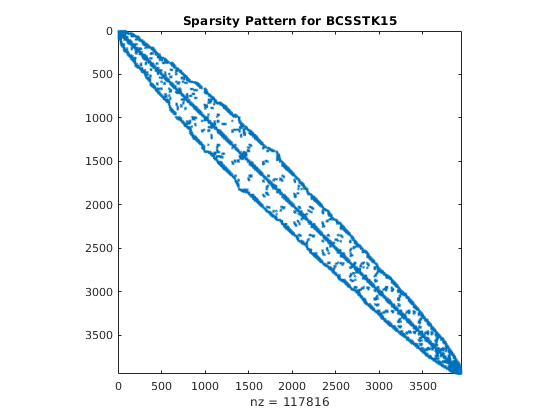
\includegraphics{lec12n-test-matrix-sparsity.png}
\caption{Sparsity pattern for BCSSTK15.}
\label{fig:lec12n-test-matrix-sparsity}
\end{marginfigure}
This matrix is not diagonally dominant\sidenote{You can visit the URL on the Matrix Market for BCSSTK15 to see a variety of matrix properties; diagonal dominance is one such property.  You can, of course, alternatively write your own function to determine whether or not a matrix is diagonally dominant.} so we might want to check the spectral radius to determine if the Jacobi method might succeed.  MATLAB code to determine spectral radius is provided in the listing below:\marginnote{
\ref{lst:ann12n-1}  The built-in function \lstinline[style=myMatlab]{eigs(A,k)} returns the $k$-largest eigenvalues of input (sparse) matrix $A$.  
}
\begin{lstlisting}[style=myMatlab]
K = -(A - diag(diag(A)));
M_inv = sparse(diag(1./diag(A)));

rho = abs(eigs(M_inv*K,1)); /*!\annotation{lst:ann12n-1}!*/
fprintf('Spectral radius of R: %g \n',rho);
\end{lstlisting}
For BCSSTK15, $\rho(A) \approx 3.17$, so we expect the un-preconditioned Jacobi method to fail---and, indeed, it does.  

Suppose we take an extreme approach and use the complete LU factorization as a preconditioner.  \marginnote[1.75cm]{
\ref{lst:ann12n-2} \lstinline[style=myMatlab]{U\\(L\\A)} is equivalent to $U^{-1}L^{-1}A$ and \lstinline[style=myMatlab]{U\\(L\\b)} is equivalent to $U^{-1}L^{-1}b$.  Recall, if $A=LU$, $A^{-1}=U^{-1}L^{-1}$.
}
\begin{lstlisting}[style=myMatlab]
[L,U] = lu(A);
nnzL = nnz(L); nnzU = nnz(U);

PA = U\(L\A); Pb = U\(L\b); /*!\annotation{lst:ann12n-2}!*/

[x_jac2,norm_res2,num_iter2,exit_code2] = ...
    jacobi_solver(PA,Pb,x_in,tol,imax);
if exit_code2 == 1
   fprintf('Preconditioned Jacobi solution successful! \n');
   fprintf('Number of iterations: %d \n',num_iter2);
   fprintf('tol = %g \n',norm_res2);
end
\end{lstlisting}
The output is shown in Figure \ref{fig:lec12n-ex1-lu-precon-out}.  Note the spectral radius of $R$ is near zero and we converged to the solution right away.\sidenote[][-2.5cm]{The only reason 2 iterations were used is because the stopping criterion was based on $|x^{(k+1)}-x^{(k)}|$ and $x^{(0)}$ was far from the solution.}
\begin{marginfigure}
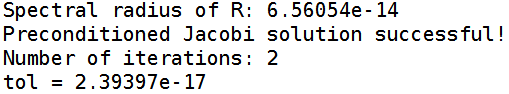
\includegraphics{lec12n-ex1-lu-precon-out.png}
\caption{Output for preconditioning with \emph{complete} LU factorization.}
\label{fig:lec12n-ex1-lu-precon-out}
\end{marginfigure}
The bad news for this example is that, while \lstinline[style=myMatlab]{A} has 117,816 non-zero entries, \lstinline[style=myMatlab]{L} and \lstinline[style=myMatlab]{U} both have on the order of a million non-zeros.  On top of that, we just performed a full LU factorization of $A$ so time spent on Jacobi iterations were wasted.

Let us now instead use an incomplete LU factorization.\marginnote[0.25cm]{
\ref{lst:ann12n-3} Use these options for \lstinline[style=myMatlab]{ilu(A,options)}. The \lstinline[style=myMatlab]{type='ilutp'} refers to incomplete LU with \emph{threshold} and \emph{pivoting} which improves the reliability of the algorithm.  The \lstinline[style=myMatlab]{droptol} is the \emph{drop tolerance} of the incomplete LU factorization.  The \emph{higher} your value of \lstinline[style=myMatlab]{droptol}, the \emph{more sparse} the resulting \lstinline[style=myMatlab]{L} and \lstinline[style=myMatlab]{U} will be; if \lstinline[style=myMatlab]{droptol} is lower, \lstinline[style=myMatlab]{L} and \lstinline[style=myMatlab]{U} will be less sparse.  In the limit, if \lstinline[style=myMatlab]{droptol=0}, then the complete LU factorization is produced. Setting \lstinline[style=myMatlab]{udiag=1} results in replacing zero diagonal entries of \lstinline[style=myMatlab]{U} with the local drop tolerance.  Selection of this option makes the \lstinline[style=myMatlab]{ilu} algorithm more reliable.  See the MATLAB documentation for \lstinline[style=myMatlab]{ilu} for a more complete description of all available options.
}
\begin{lstlisting}[style=myMatlab]
opts_ilu.type='ilutp';
opts_ilu.droptol=1e-4; /*!\annotation{lst:ann12n-3}!*/
opts_ilu.udiag=1;
[iL,iU] = ilu(A,opts_ilu);
nnz_iL = nnz(iL); nnz_iU = nnz(iU);

iPA = iU\(iL\A); iPb = iU\(iL\b);/*!\annotation{lst:ann12n-4}!*/

[x_jac3,norm_res3,num_iter3,exit_code3] = ...
    jacobi_solver(iPA,iPb,x_in,tol,imax);
if exit_code3 == 1
   fprintf('Preconditioned Jacobi solution successful! \n');
   fprintf('Number of iterations: %d \n',num_iter3);
   fprintf('tol = %g \n',norm_res3);
end
\end{lstlisting}

\vspace{0.25cm}

\noindent \ref{lst:ann12n-4} This is done for illustration purposes only.  Even if \lstinline[style=myMatlab]{iL} and \lstinline[style=myMatlab]{iU} are sparse with a low number of non-zeros, \lstinline[style=myMatlab]{iPA} and \lstinline[style=myMatlab]{iPb} will be full.  Built-in methods can use \lstinline[style=myMatlab]{iL} and \lstinline[style=myMatlab]{iU} without sparsity-destroying operations like this.
The output is shown in Figure \ref{fig:lec12n-ex1-ilu-precon-out1}.  In this case, the spectral radius of $R$ is higher but still less than 1 and, as expected, the number of required iterations to satisfy our solution tolerance is also higher.  Unlike as was the case with the complete LU factorization, the output matrices \lstinline[style=myMatlab]{iL} and \lstinline[style=myMatlab]{iU} are much more sparse, with a total number of roughly 600,000 non-zeros.  
\begin{marginfigure}
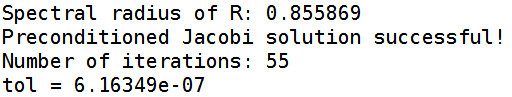
\includegraphics{lec12n-ex1-ilu-precon-out1.png}
\caption{Output for Jacobi iteration with incomplete LU preconditioning.}
\label{fig:lec12n-ex1-ilu-precon-out1}
\end{marginfigure}
If we \emph{increase} the drop tolerance to \lstinline[style=myMatlab]{opts_ilu.droptol=5e-4} we can further reduce the number of non-zeros in \lstinline[style=myMatlab]{iL} and \lstinline[style=myMatlab]{iU} to about 400,000 at the expense of increasing the spectral radius to 0.98 and, as expected, increasing the number of iterations required to reach our stopping criterion to 344.

\section{MATLAB Built-In Iterative Solvers}
There are numerous iterative solvers built into MATLAB.  We will mention only two of them and, sadly, treat them essentially as black-boxes.   
\begin{enumerate}
\item \lstinline[style=myMatlab]{pcg} - preconditioned conjugate gradient method.  
\item \lstinline[style=myMatlab]{gmres} - generalized minimum residuals method.
\end{enumerate}
Both of these algorithms are examples of Krylov subspaces methods, the details of which are beyond the scope of this class. We will use \lstinline[style=myMatlab]{pcg} for linear systems that are symmetric and positive definite.  We will use \lstinline[style=myMatlab]{gmres} for all other methods.  

\subsection{Preconditioned Conjugate Gradient}
The preconditioned conjugate gradient algorithm is one of the most competitive methods for use with sparse, symmetric matrices that are positive definite.  An excellent and easy to read description is available in the open literature.\cite{shewchuk1994conjugate}  Since \lstinline[style=myMatlab]{A} is symmetric, we can use a slightly more efficient algorithm to construct the preconditioning matrix---the incomplete Cholesky factorization: \lstinline[style=myMatlab]{ichol(A,options)}.  An example in its use is shown in the listing below:\marginnote{

\noindent \ref{lst:ann12n-5} See the MATLAB documentation for \lstinline[style=myMatlab]{ichol} for more information on these options.  The option: \lstinline[style=myMatlab]{type='ict'} directs usage of the incomplete Cholesky with threshold dropping.  This option along with \lstinline[style=myMatlab]{droptol} affects the extent to which non-zeros in \lstinline[style=myMatlab]{L} are dropped or retained.  As with \lstinline[style=myMatlab]{ilu()}, \lstinline[style=myMatlab]{droptol=0} results in a full Cholesky factorization.  The option \lstinline[style=myMatlab]{michol='on'} indicates that the modified incomplete Cholesky factorization is to be performed, use of which improves the reliability of the algorithm.
}
\begin{lstlisting}[style=myMatlab]
%% preconditioned conjugate gradient
opts.type = 'ict';
opts.droptol = 1e-4;  /*!\annotation{lst:ann12n-5}!*/
opts.michol = 'on';
L = ichol(A,opts);
[x1,fl1,rr1,it1,rv1] = pcg(A,b,tol,imax,L,L'); /*!\annotation{lst:ann12n-6}!*/

if fl1 == 0
    fprintf('pcg with ichol preconditioner solution successful!\n');
    fprintf('Residual norm: %g, after %d iterations.\n',...
        rr1,it1);
end
\end{lstlisting}

\vspace{0.1cm}

\noindent \ref{lst:ann12n-6} Several of MATLAB's built-in preconditioners use \emph{left} and \emph{right} preconditioners.  As we have described them so far, we have always use a \emph{left} preconditioner.  A right preconditioner works the same way but the matrix is applied to the right:
$$APx = bP  $$
A preconditioning matrix $P$ can be broken up into a left and right preconditioning matrix: $P = P_L P_R^{\prime}$ and applied: $$P_L A P_R^{\prime} x = P_{L}bP_R^{\prime}$$
The last two arguments for \lstinline[style=myMatlab]{pcg} correspond to the left and right preconditioning matrix respectively.   

Readers are encouraged to experiment with the preconditioned conjugate gradient built-in function with different options settings to solve a sparse, symmetric, positive definite, linear system of their choice.

\subsection{Generalized Minimum Residuals}
You should use GMRES for systems that are square and non-singular.  Since the input matrix is not necessarily symmetric or positive definite, you should use \lstinline[style=myMatlab]{ilu} to generate the preconditioning matrices.  An example usage is shown in the listing below.
\begin{lstlisting}[style=myMatlab]
%% GMRES with Incomplete LU Preconditioner
opts_ilu.type='ilutp';
opts_ilu.droptol=1e-3;
restart = [];                /*!\annotation{lst:ann12n-7}!*/
maxit = min(imax,size(A,1));

[L,U] = ilu(A,opts_ilu); 
[x4,fl4,rr4,it4,rv4] = ...
    gmres(A,b,[],tol,maxit,L,U);
\end{lstlisting}
\marginnote[-2.75cm]{

\noindent \ref{lst:ann12n-7} Please see the MATLAB documentation for explanation regarding the arguments to \lstinline[style=myMatlab]{gmres}

}
